% !TeX spellcheck = de_DE
% Die erste (unkommentierte) Zeile im Dokument legt immer die
% Dokumentklasse fest
\documentclass{scrreprt} 

% Präambel:
% Einbinen von zusätzlichen Paketen. Falls für eine Datei keine Endung
% explizit angegeben wird, benutzt LaTeX '.tex'. Im Folgenden wird
% also die Datei 'edv_pakete.tex' eingebunden.
% Die erste Zeile im Dokument legt immer die Dokumentklasse fest
%\documentclass[notitlepage]{scrreprt}
    % Die wichtigsten Dokumentklassen:
    %   scrbook, scrreprt, scrartcl, beamer, standalone
    % Einige gängige Optionen für \documentclass:
    %   ngerman
    %   titlepage, notitlepage
    %   onecolumn, twocolumn
    %   oneside, twoside
    %wird in Hauptdatei festgelegt

% Präambel

% Einige KOMA-Script-Optionen
\KOMAoptions{fontsize=12pt,paper=a4}      %Schriftgröße, Papierformat
\KOMAoptions{DIV=11}                      % Parameter mit dem man den Seitenrand ändern kann
\KOMAoptions{listof=totoc}

% Hier werden einige Pakete eingebunden
\usepackage[utf8]{inputenc}               % Direkte Eingabe von ä usw. Input=Eingabe
\usepackage[T1]{fontenc}                  % Font Kodierung für die Ausgabe Font=Ausgabe
\usepackage[ngerman]{babel}               % Verschiedenste sprach-spezifische Extras, ngerman für neue deutsche Rechtschreibung, auch UK oder US möglich
\usepackage[autostyle=true]{csquotes}     % Intelligente Anführungszeichen, arbeitet mit Babel zusammen
%

\usepackage{amsmath}%Mathedarstellung
\usepackage{commath}%Mathedarstellung
\usepackage{IEEEtrantools}%IEEEeqnarray
%
\usepackage{siunitx}   % Intelligentes Setzen von Zahlen und Einheiten
\sisetup{locale = DE}  % Deutsch als locale für die Zahlen und Einheiten
%http://tex.stackexchange.com/questions/2291/how-do-i-change-the-enumerate-list-format-to-use-letters-instead-of-the-defaul

\usepackage{enumitem}%erlaubt u.A. die Aufzählung mit Buchstaben, gefunden auf http://tex.stackexchange.com/questions/2291/how-do-i-change-the-enumerate-list-format-to-use-letters-instead-of-the-defaul
%
\usepackage[varg]{txfonts}                % Schönere Schriftart, muss nach amsmath, damit keine Fehlermeldung kommt
\usepackage{graphicx} %einbinden von Figuren/Bildern
%\graphicspath{{figs/}} % Stammverzeichnis der verwendeten Bilder, muss im selben Ordner wie Hauptdatei sein
%
\usepackage[backend=biber, style=numeric, sorting=none]{biblatex}
%Verwenden von \cite in \footnote: Bibliographie drucken lassen, mehrmals kompilieren
\usepackage{hyperref}%erzeugt klickbare Elemente
\usepackage[all]{hypcap}%hyperref-befehle springen zum oberen Rand des Bildes
% Zum Einbinden von Programmcode verwenden wir das listings-Paket
\usepackage{listings}

% Für Syntax-Highlighting:
\usepackage{xcolor}
%Fuer Bilder mit gnuplot

\usepackage{color}

% Die folgenden listings-Einstellungen sind nötig, um
% deutsche Umlaute und die Tilde (~) in listings-Umgebungen
% verwenden zu können.
\lstset{
    basicstyle=\ttfamily,    
    literate={~} {$\sim$}{1} % set tilde as a literal
    {ö}{{\"o}}1
    {ä}{{\"a}}1
    {ü}{{\"u}}1
    {ß}{{\ss}}1
    {Ö}{{\"O}}1
    {Ä}{{\"A}}1
    {Ü}{{\"U}}1
}

% Farben für Code-Syntaxhighlighting und Weiteres festlegen:
\lstset{
    % Keine besondere Markierung für Leerzeichen in Codes
    showspaces=false,               
    showstringspaces=false,         
    % Farebn für Code-Kommentare und Schlüsselworte:
    commentstyle=\color{red},       % comment style
    keywordstyle=\color{blue},      % keyword style
    stringstyle=\color{orange},		% string style
    breaklines=true,
    numbers=left,                    % where to put the line-numbers; possible values are (none, left, right)
    numbersep=5pt,                   % how far the line-numbers are from the code
    stepnumber=5, 					%how often there are line numbers in code listings
    tabsize=4, 						%default tabsize set to 4 spaces
    %language=python,
    }
%gefunden auf https://en.wikibooks.org/wiki/LaTeX/Source_Code_Listings
%eigene Kommandos/Abürzungen
\newcommand{\tb}{\textbackslash}
\newcommand{\txt}{\texttt}

%Soll Zeilenumbrueche in Gleichungen vermeiden
\binoppenalty=9999
\relpenalty=9999


% Verzeichnisse mit Abbildungen; kann gestrichen werden,
% falls Sie dies schon in edv_pakete.tex definiert haben:
\graphicspath{{Bilder/}, {Bilder/Gitter/}}
\addbibresource{refsgrosschristiane.bib}

\usepackage{textcomp}
\usepackage{eurosym}

%\addbibresource{refs.bib} %Hinzufügen einer Literaturdatenbank aus dem angegebenen Verzeichnis

% Titel, Autor und Datum
\title{Monte-Carlo Simulation eines statistischen Modells auf einem Parallelrechner}
\subtitle{Bachelorarbeit in Physik}
\date{vorgelegt der Mathematisch-Naturwissenschaftlichen Fakultät der Universität Bonn \\ Juli 2020}
\author{Christiane Franziska Groß\\ angefertigt im Helmholtz-Institut für Strahlen- und Kernphysik}

% Jetzt startet das eigentliche Dokument
\begin{document}
	\maketitle
	
	% Römische Zahlen für die Seitennummern des Inhaltsverzeichnisses
	\pagenumbering{roman}
	
	Ich versichere, dass ich diese Arbeit selbstständig verfasst habe und keine anderen als die angegebenen Quellen und Hilfsmittel benutzt sowie die Zitate kenntlich gemacht habe.

	\vspace{2cm}
	
	....................................................................................
	
	\vspace{5cm}	
	
	1. Gutachter: Prof. Carsten Urbach
	
	2. Gutachter: 
	
	\newpage
	
	% Inhaltsverzeichnis kommt hier
	\tableofcontents
	
	\clearpage
	
	% Normale Zahlen für die Seitennummern des Fliesstextes
	\pagenumbering{arabic}
	%Inhalt
	
	\section*{Einleitung}
	
	
	Die vorliegende Arbeit befasst sich mit der Magnetisierung eines Magneten, der mit dem Ising-Modell in zwei Dimensionen simuliert wird. 
	
	Dazu wird erst eine kleine Einführung in die Terminologie des Ising-Modells, von Monte-Carlo-Simulationen und möglichem Aufbau von Parallelrechnern gegeben.
	
	Danach wird erläutert, wie das Modell implementiert wurde, und wie die Fehler auf die berechneten Werte bestimmt wurden.
	
	Die so erhaltenen Werte für die Magnetisierung und den kritischen Punkt werden mit den Werten, die aus der Literatur erwartet werden, verglichen. Dies wird zeigen, dass die Monte-Carlo-Simulation gut für die Simulation geeignet ist.
	
	Schlussendlich wird untersucht, welche Laufzeitverbesserungen durch das Rechnen mit parallelen Strukturen erzielt werden können. 
	%Ziel der Arbeit, Fragestellung: Ist MC-Simulation dafür geeignet, mittels Ising-Modell einen Magneten zu simulieren?
	
	%Wie lässt sich die benötigte Laufzeit des Programms mit Parallelisierung optimieren?/Welche Laufzeitverbesserungen sind durch Parallelisierung nöglich?
	
	%Eher Zusammenfassung/abstract oder Einleitung ohne Beantwortung der Fragen?
	
	\chapter{Theoretischer Hintergrund}
	
	\section{Das Ising-Modell}
	Beim Ising-Modell handelt es sich um ein Modell für einen Ferromagneten mit starker uniaxialer Anisotropie \cite[S. 7]{binderheermann}. %Hierbei werden Teilchen, die Spin $\pm 1$ haben können, auf ein quadratisches Gitter mit konstantem Abstand zwischen den Teilchen verteilt. % Gitterförmige Anordnung von Spins, die Werte $\pm1$ annehmen können, in realen Applikationen endliche Länge, in Natur thermodynamischer Limes/unendlich lang. Hier: zweidimensionales Gitter.
	
	Der Hamiltonian des Systems ist dann nach \cite[S. 7]{binderheermann}:
	\begin{equation}
	H=-J\sum_{\langle i,j\rangle }s_is_j
	\label{eq:hamiltonianising}
	\end{equation}
	Wobei $\langle i,j\rangle$ alle benachbarten Paare sind, die Austauschenergie $J$ in beide Richtungen gleich und konstant ist und die Spins $S_i$ die  Werte $\pm 1$ annehmen können. Das Vorzeichen von $J$ bestimmt, ob der Magnet ferro- oder antiferromagnetisch ist. Es ist möglich, durch einen zusätzlichen Term ein äußeres Magnetefld zu simulieren, dies wurde in dieser Arbeit jedoch nicht getan.%Äußeres Magnetfeld möglich, aber hier vernachlässigt.

	
	%Erwarte einen kritischen Punkt mit Phasenübergang zweiter Ordnung. \cite{OnsagerCrystal1}
	Beim Ising-Modell in zwei Dimensionen wird ein Phasenübergng bei einer kritischen Temperatur erwartet, unterhalb derer sich der Magnet ferromagnetisch verhält\cite[vgl. ][]{peierls_1936}.
	
	Dieser befindet sich nach \cite{OnsagerCrystal1} bei \[\sinh^2\left(\frac{2J}{k_BT_c}\right) =1\]
	
	\begin{equation}
	\Leftrightarrow k_BT_c=\frac{2J}{\ln(1+\sqrt{2})}
	\label{eq:kritischetemperatur}
	\end{equation}
	wobei $T_c$ die kritische Temperatur und $k_B$ die Boltzmann-Konstante ist.
	
	%Magnetisierung: Erwartungswert der Spins, \[
	%M^2=\lim\limits_{m\to\infty}\left\langle s_i s_{i+m}\right\rangle \]
	
	Bei der Magnetisierung handelt es sich um den Erwartungswert der Spins\cite[vgl. ][S. 8]{binderheermann}:\[
	M=\frac{1}{N}\left\langle  \sum_{i=1}^{N} s_i \right\rangle 
	\]
	
	Die erwartete Magnetisierung unterhalb des kritischen Punkt ist nach \cite{YangMagnetization}, \cite{MontrollMagnetization}:
	\begin{equation} M=\left[1-\left(\sinh\left(\frac{2J}{k_BT}\right)\right)^{-4}\right]^{\frac{1}{8}}
	\label{eq:magnetisierungsgleichungliteratur}
	\end{equation}
	
	Oberhalb der kritischen Temperatur ist die Magnetisierung null \cite[Gl. 81]{MontrollMagnetization}.
	
	Es kommt hier also zu einer Unstetigkeit in der Magnetisierung.
	
	\section{Monte-Carlo Simulationen}
	Die Messwerte, an denen Interesse besteht, lassen sich nach \cite[S. 8]{binderheermann}  mit \[
	\langle A(\mathbf{x}) \rangle=\frac{1}{Z}\int A(\mathbf{x}) \exp(-H(\mathbf{x})/k_BT)\dif \mathbf{x}\]
	
	\[
	Z=\int \exp(-H(\mathbf{x})/k_BT) \dif \mathbf{x}
	\]
	berechnen, wobei $\mathbf{x}$ eine mögliche Konfiguration des Systems ist.
	
	
	Hierbei kann der Boltzmann-Faktor $p(\mathbf{x})=Z^{-1} \exp(-H(\mathbf{x})/k_BT)$ als die Wahrscheinlichkeit angesehen werden, mit der ein bestimmter Zustand auftritt\cite[vgl. ][S. 8 f.]{binderheermann}.
	
	Dies ist analytisch nicht machbar, da dieses Integral sehr hochdimensional ist und gleichzeitig viele Zustände nur einen sehr kleinen Beitrag zum Gesamtintegral leisten\cite[vgl. ][S. 9]{binderheermann}.
	
	Die Idee der Monte-Carlo-Simulationen ist es, solche Integrale zu Diskretisieren
	und über alle berechneten Zustände einen Mittelwert mit Gewichtung der einzelnen Zustände mit $p(\mathbf{x})$ zu berechnen. Alternativ können die Zustände auch so gezogen werden, dass sie von Anfang an nach $p(\mathbf{x})$ verteilt sind, dann ist bei der Bildung des Mittelwerts keine Gewichtung mehr notwendig. %und die Zustände mit mehr Gewicht öfter zu berechnen, damit sie bei der Summierung entsprechend mehr ins Gewicht fallen. Dafür werden die zu berechnenden Zustände $A$ so gezogen, dass sie nach $Z^{-1} \exp(-H_i/k_BT)$ verteilt sind.
	
	Dies wird durch den Metropolis-Algorithmus ermöglicht, entwickelt in \cite{metropolisupdate}:
	Es wird eine Veränderung des Systems mit Energieänderung $\Delta H$ vorgeschlagen, in diesem Fall die Umdrehung eines einzelnen Spins. Diese Änderung wird auf jeden Fall angenommen, wenn sie die Energie des Systems verringert, und wenn sie die Energie erhöht, wird die Änderung mit Wahrscheinlichkeit $\exp(-\Delta H/k_BT)$ angenommen.
	
	Insgesamt ist die Wahrscheinlichkeit zur Umdrehung eines Spins also $P=\min \left[1, \exp(-\Delta H/k_BT)\right]$
	
	Dies führt dazu, dass alle zu berechnenden Zustände aus den vorher berechneten generiert werden. Die Zustände bilden also eine Markovkette, es handelt sich um Markov Chain Monte Carlo (deutsche Bezeichnung?)
	
	Der erste Zustand wird zufällig generiert, befindet sich also nicht im Gleichgewicht und hat vermutlich ein sehr geringes Gewicht. Um in eine Region mit lokalen Energieminima/Hohen Gewichten zu kommen, ist erst eine Thermalisierung notwendig, das heißt, einige Updates, deren Ergebnisse nicht verwendet werden können, um einen Mittelwert zu bilden. (Zitate?)
	
%	Suche Observablen von komplexen Systemen. Problem: Zustandssumme, Observable $<A>$ nicht/nur schwer analytisch bestimmbar. \[Z=\int_{Alle Konfigurationen}\exp(-H/T)\] \[<A>=1/Z\int_{alle Konfigurationen} A\exp(-H/T)\] Generell: Integral bestimmen, nicht analytisch lösbar.
%	Idee: Diskretisiere Integral, verteile Summe nicht gleichmäßig, sondern summiere bevorzugt über Zustände, die ein höheres Gewicht haben. Zwei Funktionen Multiplizieren, Zahlen aus einer ziehen.
%%	wie Zustände generieren? Aus Zufallszahlen, nicht deterministisch, Zufallszahlen so verteilt, dass gewichtigere Zustände öfter vorkommen. Summiere über A, wobei A für Zustände mit höherem Gewicht öfter berechnet wurde.
%%	Wie Zufallszahlen generieren? Mit Markov-Kette, also aus vorherigem Zustand. Funktion zum Generieren: Metropolis-Update: Gehe von jeweils aktuellen zustand aus, schlage eine Veränderung vor(einen Spin auswählen und umdrehen), nehme an, wenn Energie kleiner wird, sonst mit Wahrscheinlichkeit $\exp(-\Delta H/T)$.
%%	
%	Am Anfang \enquote{Thermalisieren} oder Einbrennen nötig, da erst eine Region gefunden werden muss, in der die Zustände gut verteilt sind. Die Daten währen des Einbrennens werden nicht benötigt.
%	Quelle: Skript
%	\cite{binderheermann}
		
	\section{Parallelrechner}
	Parallelrechner: Durch Benutzung mehrerer Prozessorkerne oder mehrerer Computer benötigte Rechenzeit aufteilen und schneller Ergebnisse haben. Zwei Konzepte:
	\subsection{Shared Memory mit OpenMP}
	Open Multi-Processing\cite{specificationsopenmp}
	Mehrere Prozessoren greifen auf einen gemeinsamen Speicher zu, alle Prozesse können freigegebene Variablen verändern, Verhindern von Speicherproblemen durch critical-Bereiche, die nur ein Thread zu einer Zeit ausführen kann. Auch möglich, Variablen privat zu setzen, dann hat jeder Thread eine eigene Kopie der variable. Anwendung über Compiler-Pragmas\cite{tutorialopenmp}
	\subsection{MPI}
	Message Passing Interface
	Mehrere Rechner mit separatem Speicher arbeiten an einem Problem, Rechner kommunizieren untereinander.
	
	
		
	\chapter{Implementierung}
	Bei der Umsetzung ist nur ein endliches Gitter vorhanden.
	Randbedingungen: Auch für die Spins am Rande des Gitters muss es Nachbarn geben. Hier wurden periodische Randbedingungen gewählt, d.h. der Nachbar von einem Punkt am Ende einer Zeile ist der Punkt am Anfang der Zeile.
	
	Eine Messung: Bei jedem Spin wird ein Metropolis-Update durchgeführt.
	
	Akzeptanzrate: Wie viele Spins wurden bei einer Messung umgedreht? Wird bei jedem Punkt gezählt und in eine Variable geschrieben.
	
	Magnetisierung: Betrag der Summe über alle Spins im Gitter, je mehr Spins gleich ausgerichtet sind, desto stärker der nach außen sichtbare Effekt als Magnet. Nach jeder Messung bestimmt.
	
	Um Messungen zu vereinfachen: setze $k_B=1$, betrachte nur $T$.
		
	Initialisierung des Gitters: Als 1D array abspeichern, mit Mersenne Twister $\pm1$ auf das Gitter verteilen.
	Hamiltonian: berechnen über zeilenweise array durchgehen, von jedem Punkt rechten und unteren Nachbarn, periodische Randbedingungen durch modulo.
	Metropolis-Update: Nur vier Nachbarn zum Berechnen nötig, Hamiltonian wird als Parameter übergeben, daraus Änderung bei Flip, Akzeptanz wird durch 0/1 zurückgegeben. Wahrscheinlichkeit für Flip: Vergleich mit Zufallszahl zwischen null und eins.
	sweep Funktion: geht das ganze Gitter durch und führt bei jedem Punkt ein Metropolis-Update durch. Zählt wie viele Spins geflippt werden, schreibt am Ende Prozentuale Veränderungen (Akzeptanzrate) und Summe über alle Spins(Magnetisierung) in Ausgabedatei.
	
	Am Anfang Einbrennen nötig: Gitter der vorherigen Temperatur wird übergeben, N0 (=10.000) Messungen werden durchgeführt, deren Ergebnisse nicht verwendet werden, da sie zu stark variieren, Gitter nach Einbrennen wird in .txt Datei gespeichert.
	
	Danach messen: Ergebnisse werden in Ausgabedatei geschrieben.
	Aus Datei durch einlesen mit Standardschätzern naiven Mittelwert $\mu=\frac{1}{N}\sum_{i} x_i$ bilden und damit Standardabweichung $\sigma=\frac{1}{N-1}\sum_{i}(x_i-\mu)^2$ berechnen. Temperatur, Mittelwert und Varianz der Akzeptanzrate und Magnetisierung werden in Datei geschrieben.
	
	Fehler kommen durch Autokorrelation der Daten, sind also Temperaturabhängig: Beseitigung der Autokorrelation durch Blocking der Daten, also Einteilen in verschiedene Blöcke der Länge $l$, danach Bootstrapping, um Fehlerqualität zu verbessern. (Zitat?)
	Bootstrapping: zur Erzeugung eines Replikas aus Messwerten so viele Werte mit Zurücklegen ziehen, wie es Messungen gibt und daraus den arithmetischen Mittelwert bilden. Aus $r$ so gebildeten Replikas den Standardschätzer für Mittelwert und Varianz ziehen. Temperatur, $l$, Mittelwert und Varianz in Datei schreiben.
	
	So errechneter Fehler steigt mit l an, ab einer gewissen Länge bildet sich ein Plateau. Quelle: Skript.
	
	Bild Fehler in Abhängigkeit von l?
	
	Einzelne Messung dauert recht lange: Beschleunigen durch parallelisieren. 
	Strategie: Vor allem Rechenintensive Bereiche parallelisieren, z.B. sweep-funktion für Messvorgang und Replikas ziehen.
	Parallelisiert: for-Schleifen, deren Ausführungen unabhängig vom vorherigen Schleifendurchgang sind.
	
	sweep: bei zeilenweise durchgehen des Gitters von vorheriger Änderung abhängig.
	Unabhängig: Gitter wie Schachbrett sehen, Update der Schwarzen Felder hängt nur von weißen ab und umgekehrt. Aufspalten in zwei separate for-Schleifen, eine Farbe pos1+pos2 gerade, andere ungerade. Einzelne Schleifen parallelisieren, Updates von Hamiltonian/Anzahl der geänderten Variablen in eigene Zwischenvariablen, Updaten in einer critical region(nur ein Thread kann Region zu einer Zeit ausführen) am Ende der Schleife.
	
	Replikas ziehen: Gezogene Replikas werden in array geschrieben: Vollkommen unabhängig, parallelisieren der for-Schleife.
	
	Zeitersparnis Tabelle/Grafik Nummer an Kernen/Gebrauchte Zeit. Auch für einzelne Funktionen?
	Funktion parallelisiert, die Summe über das Gitter berechnet: Zeitersparnis nur 0,5\%, daher Hamiltonian, einmaliges Verteilen der Zufallszahlen auf Gitter nicht parallelisiert.
	
	Kritischer Punkt: Unstetigkeit in Magnetisierung/Pol in Ableitung erwartet, bestimmen über größte Änderung/Extremum der Ableitung der Magnetisierung: Mit 2-Punkt-Formel berechnete Ableitung, Fehler der Ableitung mit Gaußscher Fehlerfortpflanzung ermittelt.
	
	
	Main-funktion: Variablen wie T, J, N0 initialisieren, Array mit verwendeten Temperaturen und l fürs Bootstrapping erzeugen, Dateien für Mittelwerte öffnen
	Messungen für verschiedene Temperaturen: Durch for-Schleife, vorher Initialisierung eines Array, in das die Temperaturen gleichmäßig verteilt hineingeschrieben werden.
	Initialisierung mit (100.000) Messungen am ersten Gitter, danach Thermalisierung mit Gitter der vorherigen Temperatur.
	for-Schleife über alle Temperaturen im array: Datei für Gitter, Messergebnisse öffnen, thermalisieren, messen, naive Schätzer und Bootstrapschätzer für verschiedene l bestimmen.
	Am Ende Ableitung in separate Datei schreiben.
	
	
	 	
	\chapter{Ergebnisse}
	Parallelisierung funktioniert: Hamiltonian mit und ohne Parallelisierung gleich (Bild). siehe Bild \ref{fig:vergleichham}
	
	\begin{figure}[htbp]
		% GNUPLOT: LaTeX picture with Postscript
\begingroup
  \makeatletter
  \providecommand\color[2][]{%
    \GenericError{(gnuplot) \space\space\space\@spaces}{%
      Package color not loaded in conjunction with
      terminal option `colourtext'%
    }{See the gnuplot documentation for explanation.%
    }{Either use 'blacktext' in gnuplot or load the package
      color.sty in LaTeX.}%
    \renewcommand\color[2][]{}%
  }%
  \providecommand\includegraphics[2][]{%
    \GenericError{(gnuplot) \space\space\space\@spaces}{%
      Package graphicx or graphics not loaded%
    }{See the gnuplot documentation for explanation.%
    }{The gnuplot epslatex terminal needs graphicx.sty or graphics.sty.}%
    \renewcommand\includegraphics[2][]{}%
  }%
  \providecommand\rotatebox[2]{#2}%
  \@ifundefined{ifGPcolor}{%
    \newif\ifGPcolor
    \GPcolortrue
  }{}%
  \@ifundefined{ifGPblacktext}{%
    \newif\ifGPblacktext
    \GPblacktextfalse
  }{}%
  % define a \g@addto@macro without @ in the name:
  \let\gplgaddtomacro\g@addto@macro
  % define empty templates for all commands taking text:
  \gdef\gplbacktext{}%
  \gdef\gplfronttext{}%
  \makeatother
  \ifGPblacktext
    % no textcolor at all
    \def\colorrgb#1{}%
    \def\colorgray#1{}%
  \else
    % gray or color?
    \ifGPcolor
      \def\colorrgb#1{\color[rgb]{#1}}%
      \def\colorgray#1{\color[gray]{#1}}%
      \expandafter\def\csname LTw\endcsname{\color{white}}%
      \expandafter\def\csname LTb\endcsname{\color{black}}%
      \expandafter\def\csname LTa\endcsname{\color{black}}%
      \expandafter\def\csname LT0\endcsname{\color[rgb]{1,0,0}}%
      \expandafter\def\csname LT1\endcsname{\color[rgb]{0,1,0}}%
      \expandafter\def\csname LT2\endcsname{\color[rgb]{0,0,1}}%
      \expandafter\def\csname LT3\endcsname{\color[rgb]{1,0,1}}%
      \expandafter\def\csname LT4\endcsname{\color[rgb]{0,1,1}}%
      \expandafter\def\csname LT5\endcsname{\color[rgb]{1,1,0}}%
      \expandafter\def\csname LT6\endcsname{\color[rgb]{0,0,0}}%
      \expandafter\def\csname LT7\endcsname{\color[rgb]{1,0.3,0}}%
      \expandafter\def\csname LT8\endcsname{\color[rgb]{0.5,0.5,0.5}}%
    \else
      % gray
      \def\colorrgb#1{\color{black}}%
      \def\colorgray#1{\color[gray]{#1}}%
      \expandafter\def\csname LTw\endcsname{\color{white}}%
      \expandafter\def\csname LTb\endcsname{\color{black}}%
      \expandafter\def\csname LTa\endcsname{\color{black}}%
      \expandafter\def\csname LT0\endcsname{\color{black}}%
      \expandafter\def\csname LT1\endcsname{\color{black}}%
      \expandafter\def\csname LT2\endcsname{\color{black}}%
      \expandafter\def\csname LT3\endcsname{\color{black}}%
      \expandafter\def\csname LT4\endcsname{\color{black}}%
      \expandafter\def\csname LT5\endcsname{\color{black}}%
      \expandafter\def\csname LT6\endcsname{\color{black}}%
      \expandafter\def\csname LT7\endcsname{\color{black}}%
      \expandafter\def\csname LT8\endcsname{\color{black}}%
    \fi
  \fi
    \setlength{\unitlength}{0.0500bp}%
    \ifx\gptboxheight\undefined%
      \newlength{\gptboxheight}%
      \newlength{\gptboxwidth}%
      \newsavebox{\gptboxtext}%
    \fi%
    \setlength{\fboxrule}{0.5pt}%
    \setlength{\fboxsep}{1pt}%
\begin{picture}(8640.00,6480.00)%
    \gplgaddtomacro\gplbacktext{%
      \csname LTb\endcsname%
      \put(946,704){\makebox(0,0)[r]{\strut{}$-2.2$}}%
      \put(946,1316){\makebox(0,0)[r]{\strut{}$-2$}}%
      \put(946,1929){\makebox(0,0)[r]{\strut{}$-1.8$}}%
      \put(946,2541){\makebox(0,0)[r]{\strut{}$-1.6$}}%
      \put(946,3153){\makebox(0,0)[r]{\strut{}$-1.4$}}%
      \put(946,3766){\makebox(0,0)[r]{\strut{}$-1.2$}}%
      \put(946,4378){\makebox(0,0)[r]{\strut{}$-1$}}%
      \put(946,4990){\makebox(0,0)[r]{\strut{}$-0.8$}}%
      \put(946,5603){\makebox(0,0)[r]{\strut{}$-0.6$}}%
      \put(946,6215){\makebox(0,0)[r]{\strut{}$-0.4$}}%
      \put(1078,484){\makebox(0,0){\strut{}$0$}}%
      \put(2511,484){\makebox(0,0){\strut{}$1$}}%
      \put(3944,484){\makebox(0,0){\strut{}$2$}}%
      \put(5377,484){\makebox(0,0){\strut{}$3$}}%
      \put(6810,484){\makebox(0,0){\strut{}$4$}}%
      \put(8243,484){\makebox(0,0){\strut{}$5$}}%
    }%
    \gplgaddtomacro\gplfronttext{%
      \csname LTb\endcsname%
      \put(176,3459){\rotatebox{-270}{\makebox(0,0){\strut{}$H/\text{laenge}^2$}}}%
      \put(4660,154){\makebox(0,0){\strut{}Temperatur}}%
      \csname LTb\endcsname%
      \put(4642,6042){\makebox(0,0)[r]{\strut{}zeilenweise durchgehen}}%
      \csname LTb\endcsname%
      \put(4642,5822){\makebox(0,0)[r]{\strut{}Schachbrettmuster parallel}}%
    }%
    \gplbacktext
    \put(0,0){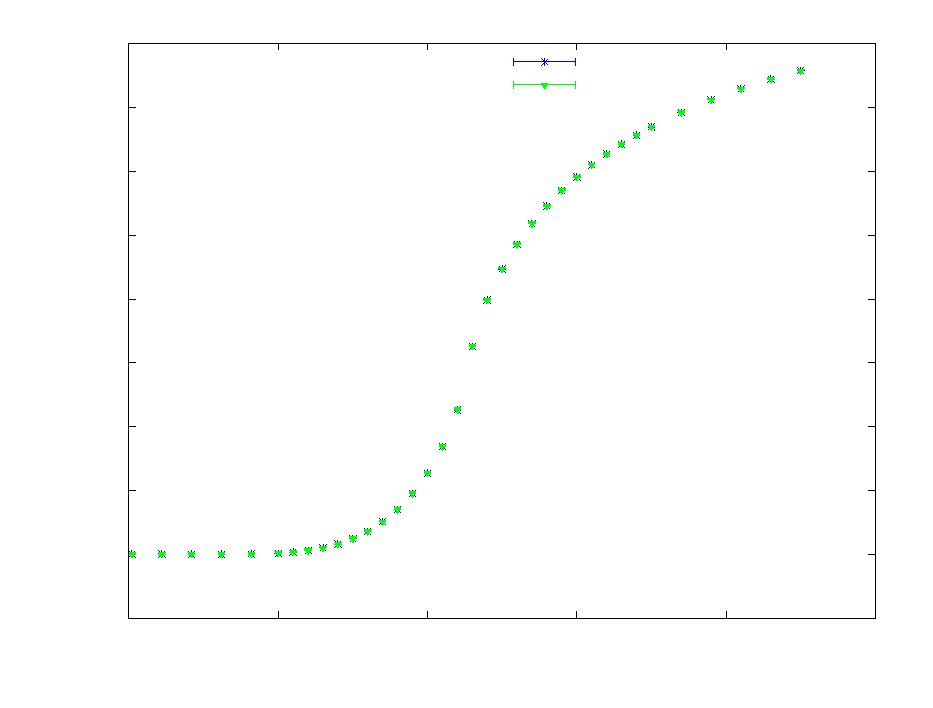
\includegraphics{vergleichham}}%
    \gplfronttext
  \end{picture}%
\endgroup

		\label{fig:vergleichham}
		\caption{Hamiltonian bei drei verschiedenen Methoden der Messreihenfolge bei verschiedenen Temperaturen}
	\end{figure}
	Akzeptanzrate: für geringe Temperaturen fast null, steigt für höhere Temperaturen, bildet Plateau? siehe Bild \ref{fig:akzeptanzratenaiv}
	
	\begin{figure}[htbp]
		\include{Bilder/akzeptanzratenaiv}
		\label{fig:akzeptanzratenaiv}
		\caption{Akzeptanzrate mit naiv berechneten Fehlern bei verschiedenen Temperaturen}
	\end{figure}
	
	Magnetisierung: Für kleine Temperaturen 1 mit geringem Fehler, wird zwischen T=1,5 und T=3 kleiner, dabei größere Fehler, bei hohen Temperaturen Magnetisierung fast null mit kleinem Fehler. Vergleich mit erwartetem Wert in Bild \ref{fig:magnetisierungbootstrap-l-128}.
	Kritischer Punkt für ${J=1:}\quad {T=2,269}$ nach Gl. \ref{eq:kritischetemperatur}, durch Ableitung (Bild) bestimmt zu $T=2,303\pm0,015$. Fehler, da kritischer Punkt in Region zwischen Wert und den nächsten Stützstellen liegen muss.
	Unterhalb kritischer Punkt: Keinen Unterschied zu Gleichung \ref{eq:magnetisierungsgleichungliteratur}. Passt gut zu Ergebnis, Verhalten wie erwartet.
	Oberhalb kritischer Punkt: weicht von Ergebnis aus Literatur ab, da Gitter endlich ist. Abweichung wird mit größerer Gitterlänge kleiner.
	
	
	\begin{figure}[htbp]
		\include{Bilder/magnetisierungbootstrap-l-128}
		\label{fig:magnetisierungbootstrap-l-128}
		\caption{Magnetisierung bei verschiedenen Temperaturen, Fehler mit Bootstrapping bei Länge 128 berechnet, Vergleich mit erwarteter Magnetisierung}
	\end{figure}
		
	Parallelisierung: Tabelle oder Bild mit Cores/Zeit.
	%Anhang
	\listoffigures
	%\listoftables
	
	
	
	\printbibliography[heading=bibintoc]
\end{document}

%\chapter{Umsetzung}
%	\section{Initialisierung und Thermalisierung}
%	Gitter, Hamiltonian, Thermalisierungsschwelle
%	
%	Gitter mit zwei for-schleifen füllen, Mersenne-Twister, der auf +-1 zugeordnet wird.
%	Hamiltonian durch Gitterdurchgang mit zwei Schleifen nach Formel \ref{eq:hamiltonianising}
%	
%	Sweep: geht gesamtes Gitter durch, führt Metropolis Update durch.
%	
%	Parallelisiert: Durchgehen in "Schachbrettmuster", erst alle schwarzen und dann alle weißen Punkte, da zum Aktualisieren der schwarzen Punkte nur alle weißen benötigt werden, somit alle Schwarzen gleichzeitig aktualisiert werden können und umgekehrt.
%	
%	Durchgang mit Schachbrettmuster dauert ca. 25 \% länger, aber beim parallelisieren geht es schon mit zwei Kernen 20 \% schneller. 
%	
%	Vergleich der Daten zeigt: Im Mittel kommt bei allen Methoden dasselbe Ergebnis heraus. \ref{fig:vergleichhamiltoniansweep}
%	
%	\begin{figure}[http]
%	\input{Bilder/Vergleichham}
%	\label{fig:vergleichhamiltoniansweep}
%		\caption{Vergleich der Mittelwerte über 10000 Messungen des Hamiltonians bei verschiedenen Methoden, das Gitter durchzugehen. Laenge=50}
%	\end{figure}
%	
%	Thermalisierung:
%	 
%	Vergleichen von hamiltonian vor und nach sweep, solange sweeps, bis Energie sich nicht mehr verringert. Bilder?
%	Geändert, da Probleme mit Springen bei der Magnetisierung auftauchen: Anfangs Thermalisierung mit vielen sweeps (10000), danach Thermalisierung auf Basis des Gitters der vorherigen Temperatur mit (5000) Sweeps
%	
%	Ausgabe mit x, y Position, Spin in txt Datei, mit gnuplot als Heatmap plotten.
%	Verhalten: Bei niedrigen Temperaturen nur ein großer, einfarbiger Bezirk, dann bei höheren Temperaturen einige Punkte mit anderer Farbe, bei hohen Temperaturen nur Rauschen.
%	
%	\begin{figure}
%	\begin{minipage}{0.48\textwidth}
%		\input{Bilder/Gitter/gitter-laenge0050-t000.tex}
%	\end{minipage}
%	\begin{minipage}{0.48\textwidth}
%		\input{Bilder/Gitter/gitter-laenge0050-t100.tex}
%	\end{minipage}
%	\begin{minipage}{0.48\textwidth}
%		\input{Bilder/Gitter/gitter-laenge0050-t250.tex}
%	\end{minipage}
%	\caption{Gitter bei verschiedenen Temperaturen}
%	\label{fig:gitter}
%	\end{figure}
%	
%	\section{Messungen}
%	\subsection{Akzeptanzrate}
%	Beim Sweep wird jede Veränderung gezählt, am Ende wird Veränderungen/laenge/laenge in Datei geschrieben. Prozentuale Veränderung.
%	Parallelisieren: Zwischenvariable für jeden Thread. Bild, erst gering, dann steil steigend, flacht ab, bildet Plateau.
%	\begin{figure}
%		\input{Bilder/akzeptanzratenaiv.tex}
%		\label{fig:akzeptanznaiv}
%		\caption{Die Akzeptanzrate bei 10000 Messungen je Temperatur mit Laenge 50}
%	\end{figure}
%	Bei welchen Temperaturen?
%	\subsection{Magnetisierung}
%	Magnetisierung= Abs(Summe über alle Spins im Gitter)
%	
%	Bilder
%	
%	-Bei kleinen Temperaturen, unterhalb von T ungefähr 0,7, ist die
%	 Magnetisierung konstant 1, mit sehr geringen Abweichungen.
%	 
%	 -Zwischen ca. 0,7 und ca. 2,5 nimmt die Magnetisierung ab, springt jedoch
%	 immer wieder zwischen stärkeren und schwächeren Magnetisierungen hin und
%	 her. Dies wird erst ab einer gewissen Gitterlänge sichtbar, bei kleineren
%	 Gitterlängen (ausprobiert habe ich es mit 10), ist die Abnahme viel weniger
%	 sprunghaft. In diesem Bereich ist die Standardabweichung der Messungen recht
%	 groß.
%	 
%	 -Bei größeren Temperaturen, oberhalb von ca. 2,5, ist die Magnetisierung
%	 annähernd konstant und fast null. Der relative Fehler ist in diesem Bereich
%	 recht groß, jedoch ist der absolute Fehler, genau wie der Messwert, klein.
%	 
%	 Behoben durch bessere Thermalisierung: bei geringeren Temperaturen konstant 1 mit geringen Fehlern, 
%	 um T=2 herum Abfall, steiler, je länger das Gitter ist, mit recht großen Fehlern, bei hohen Temperaturen konstant niedrige Magnetisierung mit größerem Fehler als bei niedriger Temperatur. (Bild)
%	 
%	 theoretischer Kritischer Punkt für $J=1:\quad T=2,269$
%	 Bestimmung: Unstetigkeit in Magnetisierung bei kritischem Punkt erwartet, d.h. Pol in der Ableitung. 
%	 Mit 2-Punkt-Formel Ableitung bestimmen, Extremum: kritischer Punkt muss zwischen den beiden Nachbarn liegen. Ergebnis für l=128: Kritischer Punkt bei $T=2,303\pm0,015$.
%	 	\begin{figure}
%	 		\input{Bilder/ableitung.tex}
%	 		\label{fig:ableitung}
%	 		\caption{Ableitung der Daten aus l=128 mit 2-Punkt-Formel}
%	 	\end{figure}
%	 	
%	 
%	 Temperatur durch Autokorrelation, durch Bootstrapping mit blocking ausgleichen. 
%	 Zuerst Fehler, da Replika falsch verstanden, danach klare Änderung vom Fehler mit l (Bild).
%	 
%	 Magnetisierung mit Bootstrap: Bild, kleinerer Fehler, Fehler bei Phasenübergang größer als darunter/darüber.
%	\begin{figure}
%		\input{Bilder/magnetisierungbootstrap-l-128.tex}
%		\label{fig:magnetisierungbootstrap-l-128}
%		\caption{Die Magnetisierung bei 10000 Messungen je Temperatur mit Laenge 50, Bootstrapping von Daten mit Blocklänge 128}
%	\end{figure}
%		
%	Parallelisieren, indem Replica parallel gezogen werden, jedes Replica in array geschrieben, danach nur Mittelwert und Varianz über Array berechnen.
%	Vergleich: Mittelwerte gleich.
%	\begin{figure}
%		\input{Bilder/vergleichbootstrap-l-128.tex}
%		\label{fig:bootstrapparallel-l-128}
%		\caption{Die Magnetisierung bei 10000 Messungen je Temperatur mit Laenge 50, Bootstrapping von Daten mit Blocklänge 128, Vergleich von parallel und nicht paralleler Funktion}
%	\end{figure}	
